\documentclass[a4paper,12pt]{article}

\usepackage{graphicx}
\usepackage{hyperref}
\usepackage{multibib}
\usepackage{fancyhdr}
\usepackage{float}

\usepackage{tikz}
\usetikzlibrary{arrows,automata,positioning,matrix}
\usepackage[pdftex]{pict2e}
\usepackage[top=1.25in,bottom=1.25in,left=1.5in,right=1.25in]{geometry}

\fancyhf{} % clear all header and footers
\renewcommand{\headrulewidth}{0pt} % remove the header rule
\rfoot{\thepage}

\newcites{bib}{Bibliography}
\newcites{ref}{References}
\bibliographystyle{apalike}


\pagestyle{fancy}
\begin{document}
\setcounter{secnumdepth}{4} %so that we get subsubsubsection
\setcounter{tocdepth}{4} %so that subsubsubsection get's shown on Table of contents

\begin{center}
    \pagenumbering{gobble}
    \textbf{\Large Kathmandu University} \\[0.3cm]
    \textbf{\large Department of Computer Science and Engineering} \\[0.3cm]
    \textbf{\Large Dhulikhel,Kavre} \\[0.8cm]

    \includegraphics[width=0.3\textwidth]{images/ku.jpg} \\[0.6cm]


    \textbf{\large A Project Report} \\[0.3cm]
    \textbf{\large on} \\[0.6cm]
    { \huge \bfseries “FPGA Console”} \\[0.3cm]

    { \large \bfseries COMP 342} \\[0.3cm]

    { \normalsize \bfseries for  partial fullfullment of III/II in Computer Science/Engineering} \\[0.6cm]

    \textbf{\large Submitted By} \\[0.2cm]

    \textbf{\large Ashish Thapa(56)}

    \textbf{\large Aditya Jha(20)} \\[1.2cm]

    \textbf{\large Submitted To} \\[0.2cm]
    \textbf{\large Dr. Rajani Chulyadyo} \\[0.2cm]
    \textbf{\large Department of Computer Science and Engineering} \\[1.5cm]


    \textbf{\large Submission Date:} \\[0.3cm]
    \today
\end{center}

    \newpage
    \vspace*{2cm}
    \begin{center}
    \section*{Bonafide Certificate}
    \pagenumbering{Roman}
    \addcontentsline{toc}{section}{Bonafide Certifate}
    \vspace{2cm}
    \textbf{\large This project Work on} \\[0.2cm]
    \textbf{\large “FPGA Console”} \\[0.2cm]
    \textbf{\large is the bonafide work of} \\[0.2cm]
    \textbf{\large “Ashish Thapa, Aditya Jha”} \\[0.2cm]
    \textbf{\large who carried out the project work under my supervision} \\[0.2cm]
    \end{center}

    \vspace{3cm}
    \phantom{} \\[0.2cm]
    \textbf{\large Project Supervisor}
    \phantom{} \\[0.2cm]
    \rule{6cm}{0.1pt} \\[0.2cm]
    \textbf{\large Name: Dr. Sudan Jha} \\[0.2cm]
    \textbf{\large Academic Designation: Professor}

    \newpage
    \section*{Abstract}
    \addcontentsline{toc}{section}{Abstract}


    FPGA technology has been widely used in digital systems, especially in embedded systems. Tang Nano 9k is a low-cost FPGA board that can be used to implement digital systems. The aim of this project is to create a custom CPU focused to act as a brain for a game console using Tang Nano 9k FPGA board. This project aims to provide hands-on experience with FPGA development and custom ISA implementation.The project uses open source tools for digital design like Yosys,synth\_gowin,next pnr-gowin,iverilog, GTKWave etc. The project includes the development of a CPU with a custom ISA, buttons as  input device, SSD1306 OLED as a output device, and ESP8266 as a display controller. Various protocols like UART, SPI, and I2C are used to communicate with various modules within the fpga console. The outcome of this project is a working game console where assembly code for games like pong can be loaded into the flash and played. The project has provided a better understanding of communication interface, fpga toolchain and implementation of custom ISA.This project can be extended to include more advanced features such as networking capabilities, sound output, and additional input devices. 
    \vspace{0.5cm}

    \noindent
    \textbf{Keywords}: \textit{FPGA technology, game console,, Yosys, nextpnr-gowin, GTKWave, custom CPU, ,UART, SPI, assembly}

    \newpage
    \pagenumbering{gobble}
    \tableofcontents

    % defining list of figures and list of tables

    \newpage
    \listoffigures
    \addcontentsline{toc}{section}{List of Figures}
    \pagenumbering{Roman}
    \setcounter{page}{3}

    \newpage
    \listoftables
    \addcontentsline{toc}{section}{List of Tables}
    \newpage

    % abbreviation

    \section*{Abbreviation} 
    \addcontentsline{toc}{section}{Abbreviation}
    \renewcommand{\arraystretch}{2.3}
    \label{tab:acronyms}
    \begin{tabular}{|c|p{0.7\linewidth}|}
    \hline
    \textbf{Acronym} & \textbf{Description} \\
    \hline
    FPGA & Field-Programmable Gate Array \\
    ISA & Instruction Set Architecture \\
    OLED & Organic Light Emitting Diode \\
    ESP & Electronic Stability Program \\
    UART & Universal Asynchronous Receiver-Transmitter \\
    SPI & Serial Peripheral Interface \\
    I2C & Inter-Integrated Circuit \\
    CPU & Central Processing Unit \\
    VGA & Video Graphics Array \\
    HDL & Hardware Description Language \\
    DSA & Domain Specific Architecture\\
    RISC & Reduced Instruction Set Architecture\\
    CISC & Complex Instruction Set Architecture\\
    \hline
    \end{tabular}

    % main matter
    \newpage
    \pagenumbering{arabic}
    \setcounter{page}{1}
    \section{Introduction}
    \subsection{Background}

    \phantom{}

    Field Programmable Gate Arrays (FPGA) are integrated circuits that can be programmed to perform any digital function by configuring the interconnects and logic gates inside the chip. They are different from processors or microcontrollers as FPGA contains logic blocks and look up tables that are placed and routed , which means there is no instruction set and fetching, decoding or executing. It can be optimized for specific tasks and it allows parallel processing .Since its inception in Xilinx has seen rapid growth and adoption mainly because of its high configurability and flexibility. 

    Since FPGA performance is comparable to real digital circuit, and the toolchain it comes bundled with allows easy testing and prototyping. Building the CPU with custom Instruction set becomes relatively easy. A CPU has a predefined set of instructions one can use to program it. Those instructions or Instruction set architecture are of two types i.e  Complex Instruction Set Architecture(CISC) and Reduced Instruction Set Architecture(RISC). RISC has limited number of instruction set and simpler microarchitecture. RISC-V contains 32-bit integer instruction set called \textbf{RV32I}, which includes 47 instructions only \citebib{arvindpdmn_risc-v_2018}. Other Popular Instruction set architectures are x86, ARM , MIPS, Xtensia etc. 

    Gaming Consoles have been around 1970s and has evolved significantly over the years. The first game console, Magnavox Odyssey, was released in 1972 was a simple analog device. Today consoles like PS5, Xbox, Nintendo Switch are sophisticated devices with advanced features. %%\citebib{cite world history here} %.
    The project aim is to create a simple enough game console using an FPGA which offers flexibility and customization. This approach allows us total control over how the console is designed. The Instruction set architecture can be specifically designed to cater console devices. 

    \subsection{Objectives}
    \begin{itemize}
        \item To create a simple game console using the FPGA, with simple input and output devices.
        \item To Design and implement our own CPU with custom Instruction Set Architecture(ISA) which can be used to write the games for the console
        \item To understand and use various hardware communication interfaces like UART, SPI , $I^2C$
        \item To develop proficiency in programming with Hardware Description language(HDL) like Verilog  
    \end{itemize}

    \subsection{Motivation and Significance}
    FPGAs are highly versatile programmable devices which can perform any digital function. It also generally supports large array of input/output pins which can interface with other deivces. The motivation for this project is to create a custom game console from scratch using FPGA technology, with a focus on developing a CPU with a custom instruction set architecture (ISA) and implementing it in hardware. 

    Learning to create a game console or any hardware system from scratch is arduous task. Newer ones are very complex and the old ones or the simple ones either have a closed system architecture or requires different Integrated Circuits(ICs) which are already discontinued to be produced. For those who wants to understand how simple consoles work, there is no proper resources available. This project aims to be as simple as possible and include bare minimum number of input devices, some form of video output while documenting each and every significant part of the process. By creating a custom game console, this project provides a platform for hardware enthusiast to experiment and create new games with a custom instruction set architecture while utilizing parallelization of FPGAs.

    This project is different from existing works in that it focuses on creating a custom game console from scratch, rather than modifying an existing system. Additionally, the development of a custom ISA allows for greater flexibility and optimization of game code. The use of FPGA technology also provides the ability to modify and upgrade the hardware, enabling the console to evolve over time.

    Overall, the significance of this project lies in its potential to inspire further innovation in the field of hardware world, as well as its educational value in providing hands-on experience with FPGA technology, computer architecture, and digital circuit design.
    \newpage
    \section{Related Works}
    \subsection{Architectures}
    Starting From the 1960s, when IBM had 4 computer lines, all of them had 4 different ISAs. Custom instruction set for each computer line which had similar task was not optimal so companies moved towards a standarizing a single instruction set architecture. Intel has x86 architecture, Softbank Group owns ARM architecture, University of California Berkely manages RISC-V architecture. These exisiting architecures represents culmination of years of development and is suitable for various kinds of tasks.
    Custom Instruction set Design also has gained considerable attention in recent years. As the increasing demands for performance arises. Custom design gives total control. One example of Domain specific Architecture (DSA) is Google \textit{ Tensor Processing Unit} first deployed in 2015. 
    \subparagraph{RISC-V}
    It is one of the opensource General purpose specification that can run operating systems, compilers and so on. It has a modular architecture.It supports little endian byte ordering system. Its primary features are
    \begin{itemize}
        \item  completely open ISA which is free to academia and industry.
        \item 32-bit and 64-bit address space variants
        \item support for highly-parallel multicore or manycore implementation
    \end{itemize}
    \subparagraph{ARM}
     architecture is owned by Softbank group. First arm processor called ARM1 was developed by Acord computer in Britain for BBC. The architecture state for the ARM processor consists of 16 \textit{32-bit} registers and the status register. In 1995 it introduced the \textit{16-bit} thumb instruction set which makes the code size small but are less powerful.Later enhancement has added digital signal processing (DSP), optional floating point instructions, power saving and Single instruction Multiple data (SIMD) instructions. ARMv8 introduced a completely new 64-bit architecture. 

    \subparagraph{Google TPU}
    can run \textit{Deep Neural Network} interface 15-to-30 times faster  than contemporary CPU and GPU. \citebib{}. It can achieve such performance because
    \begin{itemize}
        \item it has large 2-dimensional multiply units compared to contemporary CPU which has 13 to 18 times smaller multiply units.
        \item it uses domain specific architecture (DSA) specifically created to decrease the cost and increase the performance. 
    \end{itemize}

    \subsection{Consoles}

    \subsubsection{Mister FPGA Project}
    Mister is an open source project that aims to recreate classic computers, video game consoles, and arcade machines using modern hardware. It uses an FPGA board called DE10-Nano which connects to TV or monitor via HDMI video out. It can also be expanded with various add-on boards such as 7-port USB hub.

    \begin{figure}[h]
    \centering
    \includegraphics[width=0.5\textwidth]{images/mister.png} 
    \caption{Mister FPGA DE10-Nano Board}
    \end{figure}

    \subsubsection{FPGA-CHIP8} 
    CHIP-8 is a virtual machine with an interpreted environment widely used in the 1970s.
    FPGA-CHIP8 implements CHIP-8 specification for TinyFPGA BX board. Other hardware components are a 16-button keyboard and 128x64px monochrome OLED screen
    \newpage
    \begin{figure}[h]
    \centering
    \includegraphics[width=0.3\textwidth]{images/chip8-fpga.png} 
    \caption{FPGA-CHIP8 running Space invaders}
    \end{figure}

    \subsubsection{FPGAboy} 
    FPGABoy is an implementation of Nintendo's classic handheld Game Boy system. It runs on Digilent Atlys board. Xilinx ISE webPACK is used as IDE and for simulations
    \begin{figure}[h]
    \centering
    \includegraphics[width=0.3\textwidth]{images/fpgaboy.png} 
    \caption{Tetris run on FPGAboy}
    \end{figure} 
    \newpage
    \section{Design and Implementation}
    \subsection{Procedure}

    \subsubsection{Learning oss-cad-suite}
    OSS CAD Suite is distribution for open source software used in digital logic design.
    There are tools for RTL synthesis, hardware verification, place and route and support for Hardware Definition Language(HDL) like Verilog. HDLBits is collection of verilog exercises suited for learning Verilog. \url{https://hdlbits.01xz.net/wiki/Special:VlgStats/216F4A6FBFA9331} contains the list of solved problems. 

    \subsubsection{Learning Communication Interfaces}
    \paragraph{Interfacing with flash memory with SPI interface}
    \paragraph{Interfacing with Screen using UART interface}
    \subsubsection{Building the CPU}
    \subsubsection{Writing Assembly Code for Games}


    \newpage

    \begin{table}[H]
    \footnotesize
    \centering
    \setlength{\tabcolsep}{0.5em} % for the horizontal padding
    {\renewcommand{\arraystretch}{1}% for the vertical padding
    \begin{tabular}{|c|l|l|l|p{6cm}|}
    \hline
    \textbf{Command} & constant & opcode & variation & description \\ \hline
    CLEAR A & 0 & 00000 & 1000000000 & clear A Register \\ \hline
    CLEAR B & 0 & 00000 & 0100000000 & clear B Register\\ \hline
    CLEAR AC & 0 & 00000 & 0010000000 & clear AC Register\\ \hline
    CLEAR BTN1 & 0 & 00001 & 1000000000 & clear AC if btn1 pressed\\ \hline
    CLEAR BTN2 & 0 & 00001 & 0100000000 & clear AC if btn2 pressed\\ \hline
    CLEAR BTN3 & 0 & 00001 & 0010000000 & clear AC if btn3 pressed\\ \hline
    CLEAR BTN4 & 0 & 00001 & 0001000000 & clear AC if btn4 pressed\\ \hline
    STA A & 0 & 00010 & 1000000000 & store AC in A register\\ \hline
    STA B & 0 & 00010 & 0100000000 & store AC in B register\\ \hline
    STA C & 0 & 00010 & 0010000000 & store AC in C register\\ \hline
    STA LED & 0 & 00010 & 0001000000 & set first 6 bits of AC register to LED output\\ \hline
    INV A & 0 & 00011 & 1000000000 & invert A register\\ \hline
    INV B & 0 & 00011 & 0100000000 & invert B register\\ \hline
    INV C & 0 & 00011 & 0010000000 & invert C register\\ \hline
    INV AC & 0 & 00011 & 0001000000 & invert AC register\\ \hline
    HLT & 0 & 00100 & 0000000000 & halt\\ \hline
    ADD A & 0 & 00101 & 1000000000 & Add A to AC register\\ \hline
    ADD B & 0 & 00101 & 0100000000 & Add B to AC register\\ \hline
    ADD C & 0 & 00101 & 0010000000 & Add C to AC register\\ \hline
    ADD 20 & 1 & 00101 & 0000000001 & Immediate Add \\ 
    &  &  & value  & \\ \hline
    SUB A & 0 & 00110 & 1000000000 & Sub A and AC register\\ \hline
    SUB B & 0 & 00110 & 0100000000 & Sub B and AC register\\ \hline
    SUB C & 0 & 00110 & 0010000000 & Sub C and AC register\\ \hline
    SUB 20 & 1 & 00110 & 0000001010 & Immediate Subtract\\ 
    &  &  & value  & \\ \hline
    PRNT A & 0 & 00111 & 1000000000 & Print A reg to OLED \\ \hline
    PRNT B & 0 & 00111 & 0100000000 & Print B reg to OLED \\ \hline
    PRNT C & 0 & 00111 & 0010000000 & Print C reg to OLED\\ \hline
    PRNT 110 & 1 & 00111 & 0110110110 & Immediate Print value to OLED\\ \hline
    RECT X Y W H & 0 & 01000 & XXXXXYYYYY & Draw rect of in pos x and y of size w and h\\ 
    & 0 & 00000 & WWWWWHHHHH &\\ \hline 
    CIRC X Y R & 0 & 01001 & XXXXXYYYYY & Draw Circle of radius R in position X and Y\\ 
    & 0 & 00000 & 00000RRRRR & \\ \hline
    PIX X Y & 0 & 01010 & XXXXXYYYYY & Draw pixel in X and Y position\\ \hline
    JMPZ A & 0 & 01100 & 1000000000 & Jump to A Register position if AC = 0\\ \hline
    JMPZ B & 0 & 01100 & 0100000000 & Jump to B Register position if AC = 0\\ \hline
    JMPZ C & 0 & 01100 & 0010000000 & Jump to C Register position if AC = 0\\ \hline
    JMPZ 20 & 1 & 01100 & 0000000001 & Immedate jump \\ 
    &  &  & value  & \\ \hline
    WAIT A & 0 & 01101 & 1000000000 & Wait for amount of seconds as specified by A register\\ \hline
    WAIT B & 0 & 01101 & 0100000000 &  Wait for amount of seconds as specified by B register\\ \hline
    WAIT C & 0 & 01101 & 0010000000 &  Wait for amount of seconds as specified by C register\\ \hline
    WAIT 20 & 0 & 01101 & 0000000001 &  Immediate Wait for amount of seconds \\ 
    &  &  & value  & \\ \hline
    \end{tabular}
    }
    \caption{Instruction set Architecture}
    \end{table}

    \newpage

    Instruction set architecture defines 
    \begin{itemize}
        \item instruction set: the function of each instruction
        \item Register set : how many registers there are , size of registers, functions and its initial state
        \item Exception Model: What are the different level of privilege 
        \item Memory Model 
    \end{itemize}
    \newpage
    \subsection{Diagrams}
    
    \begin{figure}[h]
    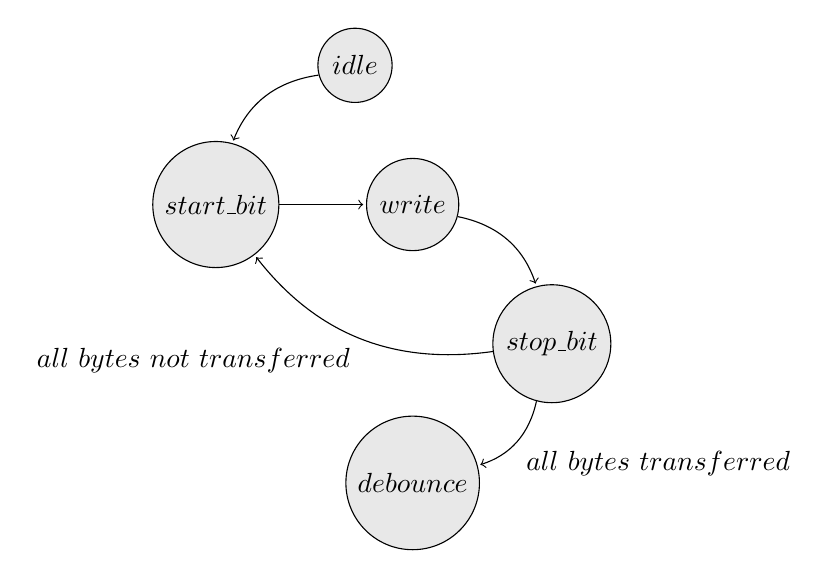
\begin{tikzpicture}[shorten >=1pt,node distance=2.5cm,auto]
    \tikzstyle{every state}=[fill={rgb:black,1;white,10}]

    \node[state]   (idle)                      {$idle$};
    \node[state] (startbit) [below left of=idle]  {$start\_bit$};
    \node[state]           (write) [right of=startbit]     {$write$};
    \node[state] (stop) [below right of=write] {$stop\_bit$};
    \node[state]           (debounce) [below left of=stop]     {$debounce$};

    \path[->]
    (idle) edge [bend right] node {} (startbit)
    (startbit) edge node {} (write)
    (write) edge [bend left] node {} (stop)
    (stop) edge [bend left] node {$all\ bytes\ not\ transferred$} (startbit)
    (stop) edge [bend left] node {$all\  bytes\ transferred$} (debounce);
    \end{tikzpicture}
    \caption{State diagram for UART Protocol} 
    \end{figure}
% SPI
    \begin{figure}[h!]
    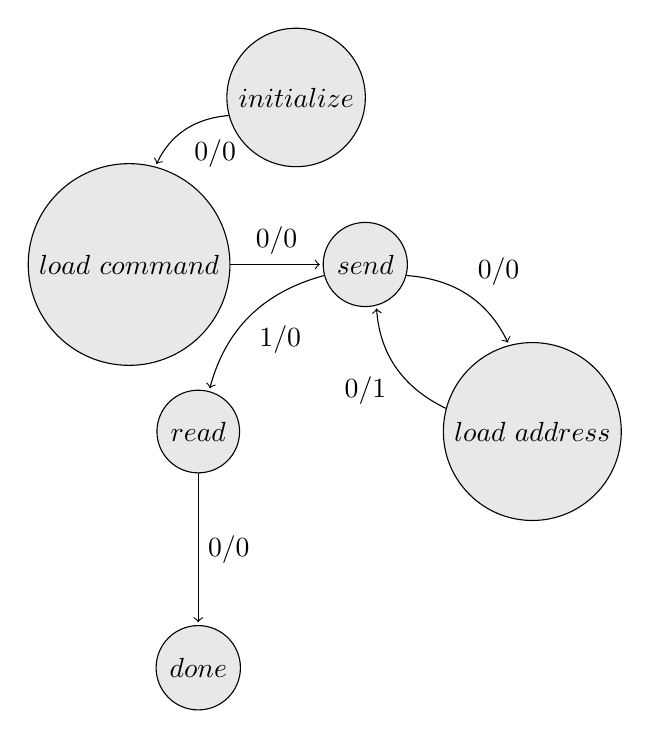
\begin{tikzpicture}[shorten >=1pt,node distance=3cm,auto]
    \tikzstyle{every state}=[fill={rgb:black,1;white,10}]

    \node[state]   (init)                      {$initialize$};
    \node[state] (loadcmd) [below left of=init]  {$load\ command$};
    \node[state]           (send) [right of=loadcmd]     {$send$};
    \node[state] (loadaddr) [below right of=send] {$load\ address$};
    \node[state]           (read) [below left of=send]     {$read$};
    \node[state]           (done) [below of=read]     {$done$};

    \path[->]
    (init) edge [bend right] node {$0/0$} (loadcmd)
    (loadcmd) edge node {$0/0$} (send)
    (send) edge [bend left] node {$0/0$} (loadaddr)
    (loadaddr) edge [bend left] node {$0/1$} (send)
    (send) edge [bend right] node {$1/0$} (read)
    (read) edge node {$0/0$} (done);
    \end{tikzpicture}
    \caption{State diagram for SPI Flash Protocol}
    \end{figure}

    \newpage

        % CPU
    \begin{figure}[H]
    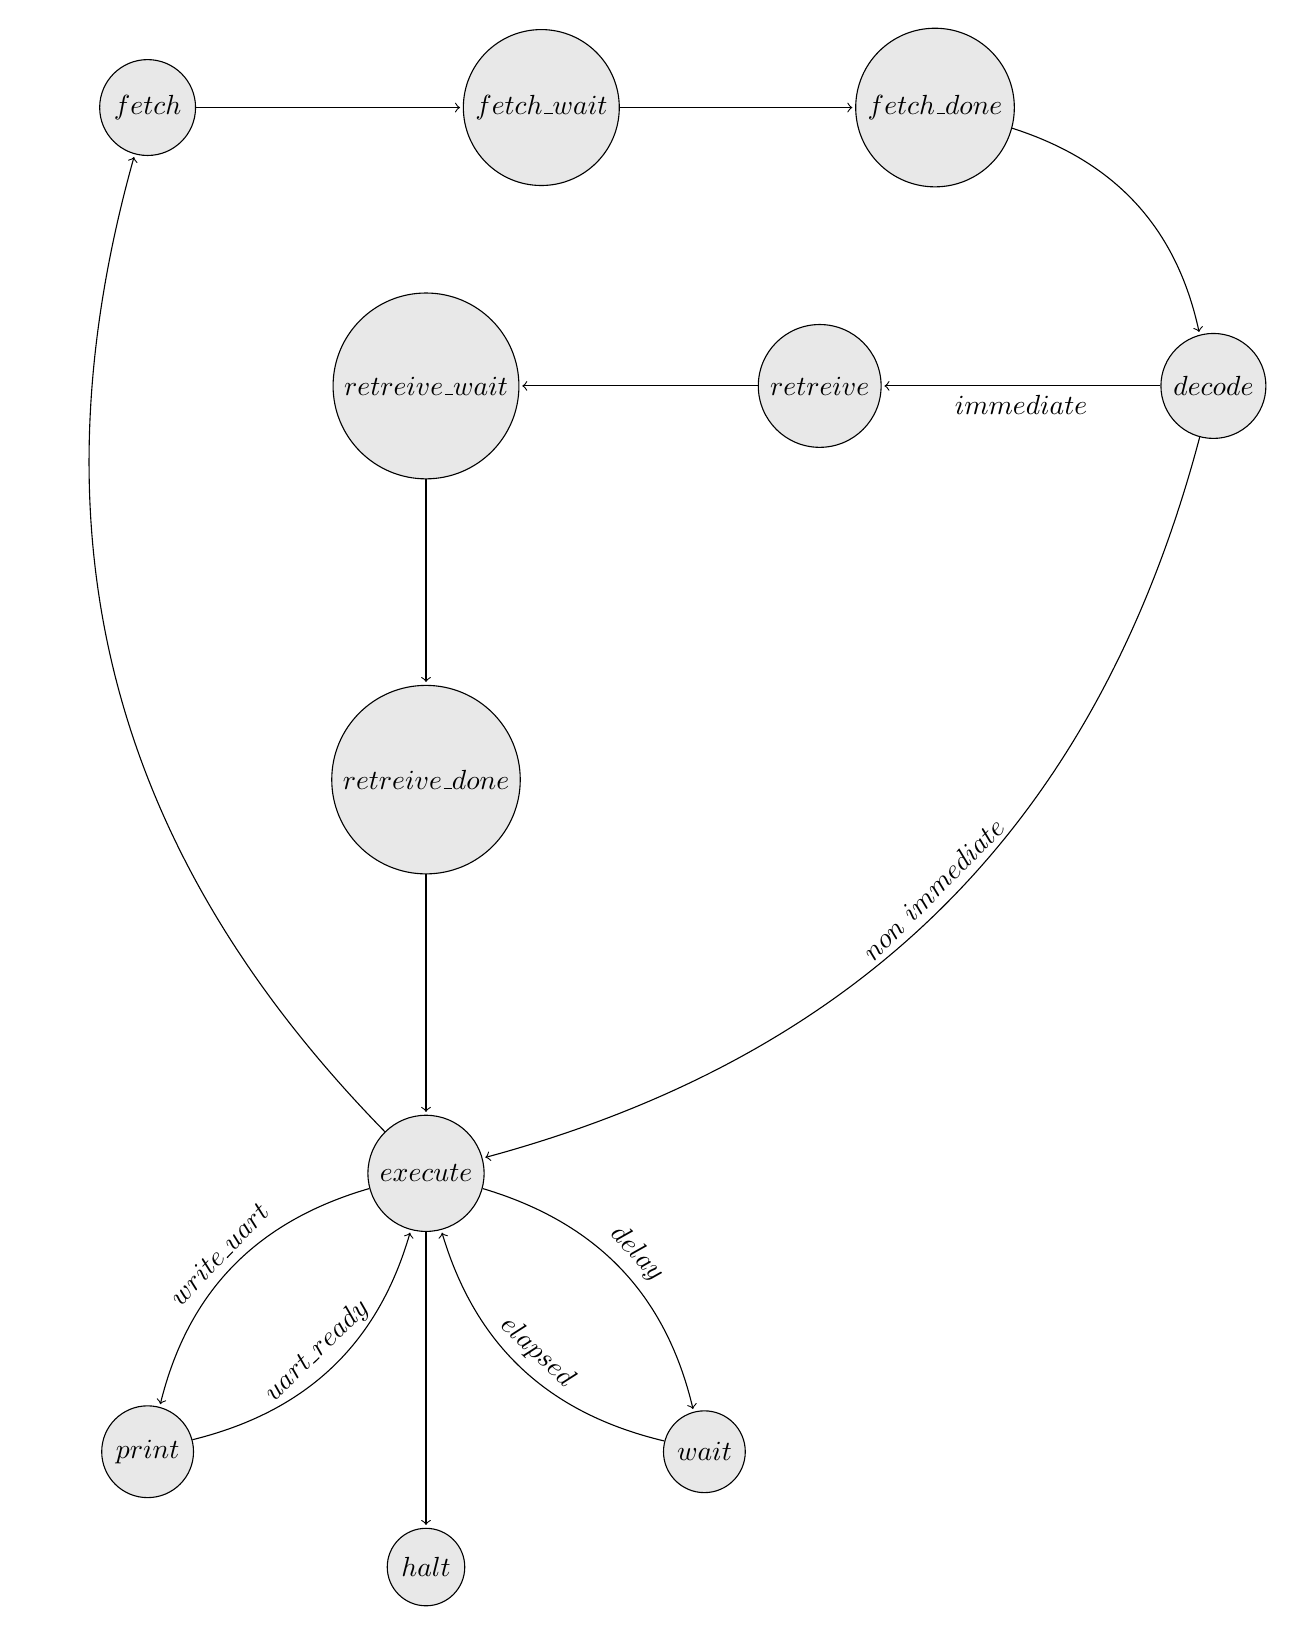
\begin{tikzpicture}[shorten >=1pt,node distance=5cm,auto]
    \tikzstyle{every state}=[fill={rgb:black,1;white,10}]

    \node[state]   (fetch)                      {$fetch$};
    \node[state] (fwait) [right of=fetch]  {$fetch\_wait$};
    \node[state]           (fdone) [right of=fwait]     {$fetch\_done$};
    \node[state] (decode) [below right of=fdone] {$decode$};
    \node[state]           (retreive) [left of=decode]     {$retreive$};
    \node[state]           (rwait) [left of=retreive]     {$retreive\_wait$};
    \node[state]           (rdone) [below of=rwait]     {$retreive\_done$};
    \node[state]           (execute) [below of=rdone]     {$execute$};
    \node[state]           (print) [below left of=execute]     {$print$};
    \node[state]           (wait) [below right of=execute]     {$wait$};
    \node[state]           (halt) [below of=execute]     {$halt$};
    \path[->]
    (fetch) edge  node {} (fwait)
    (fwait) edge  node {} (fdone)
    (fdone)  edge [bend left]  node {} (decode)
    (decode) edge  node {$immediate$}  (retreive)
    (decode) edge [bend left] node [sloped] {$non\ immediate$} (execute)
    (retreive) edge node {} (rwait)
    (rwait) edge  node {} (rdone)
    (rdone) edge  node {} (execute)
    (execute) edge [bend right]  node [sloped] {$write\_uart$} (print)
    (execute) edge [bend left]  node [sloped] {$delay$} (wait)
    (print) edge [bend right]  node [sloped] {$uart\_ready$} (execute)
    (wait) edge [bend left]  node[sloped] {$elapsed$} (execute)
    (execute) edge node {} (halt)
    (execute) edge [bend left] node {} (fetch);
    \end{tikzpicture}
    \caption{State diagram for CPU}
    \end{figure}

    \begin{figure}[h]
    \setlength{\unitlength}{0.8cm}
    \begin{picture}(16,1)
    \multiput(0,0)(0,1){2}{\line(1,0){16}}
    \multiput(0,0)(1,0){17}{\line(0,1){1}}
    \put(0,-1){\line(1,0){1}}
    \put(0,-1){\line(0,1){1}}
    \put(0.1,-0.7){$CM$}
    \put(1,-1){\line(0,1){1}}
    
    \put(1,-1){\line(1,0){5}}
    \put(1,-1){\line(0,1){1}}
    \put(1.2,-0.7){$COMMANDS$}
    \put(6,-1){\line(0,1){1}}
    
    \put(6,-1){\line(1,0){10}}
    \put(6,-1){\line(0,1){1}}
    \put(6.2,-0.7){$VARIATION$}
    \put(16,-1){\line(0,1){1}}
    \end{picture}
    \vspace{0.4cm}
    \caption{ISA}
    \end{figure}

    \subsection{System Requirement Specification}
    \subsubsection{Software specification}
    \paragraph{Verilog}
    \paragraph{Yosys}
    \paragraph{gowith-pnr}
    \subsubsection{Hardware specification}

    \newpage
    \section{Discussion on Achievements}

    \newpage
    \section{Conclusion and Recommendatation}
    \subsection{Limitation}

    \subsection{Future Enhancement}

    hello leslie lamport \citebib{Herlocker:2004}
     hello leslie lamport \citebib{HuLiu:2004}

    hello leslie lamport \citeref{opinion:lexicon}

    \bibliographystylebib{plain}
    \bibliographybib{Bibliography}

    \bibliographystyleref{plain}
    \bibliographyref{References}
\end{document}